
\begin{multicols}{3}
\begin{textbox}{Neural Networks}
\begin{subbox}{subbox}{ Introduction}
\scriptsize
Now it’s time for you to create your first neural network using PyTorch. This section will walk you through the process of:
\begin{itemize}
    \item 
Creating a simple neural network model
    \item Training the network
    \item Visualizing the results of the network
    \item Tweaking the network
\end{itemize}
\end{subbox}
\begin{subbox}{subbox}{ Data }
\scriptsize
First we need some sample data to train our network on. The example dataset consists of 2D points along two interleaving half circles, figure below. 
\centering
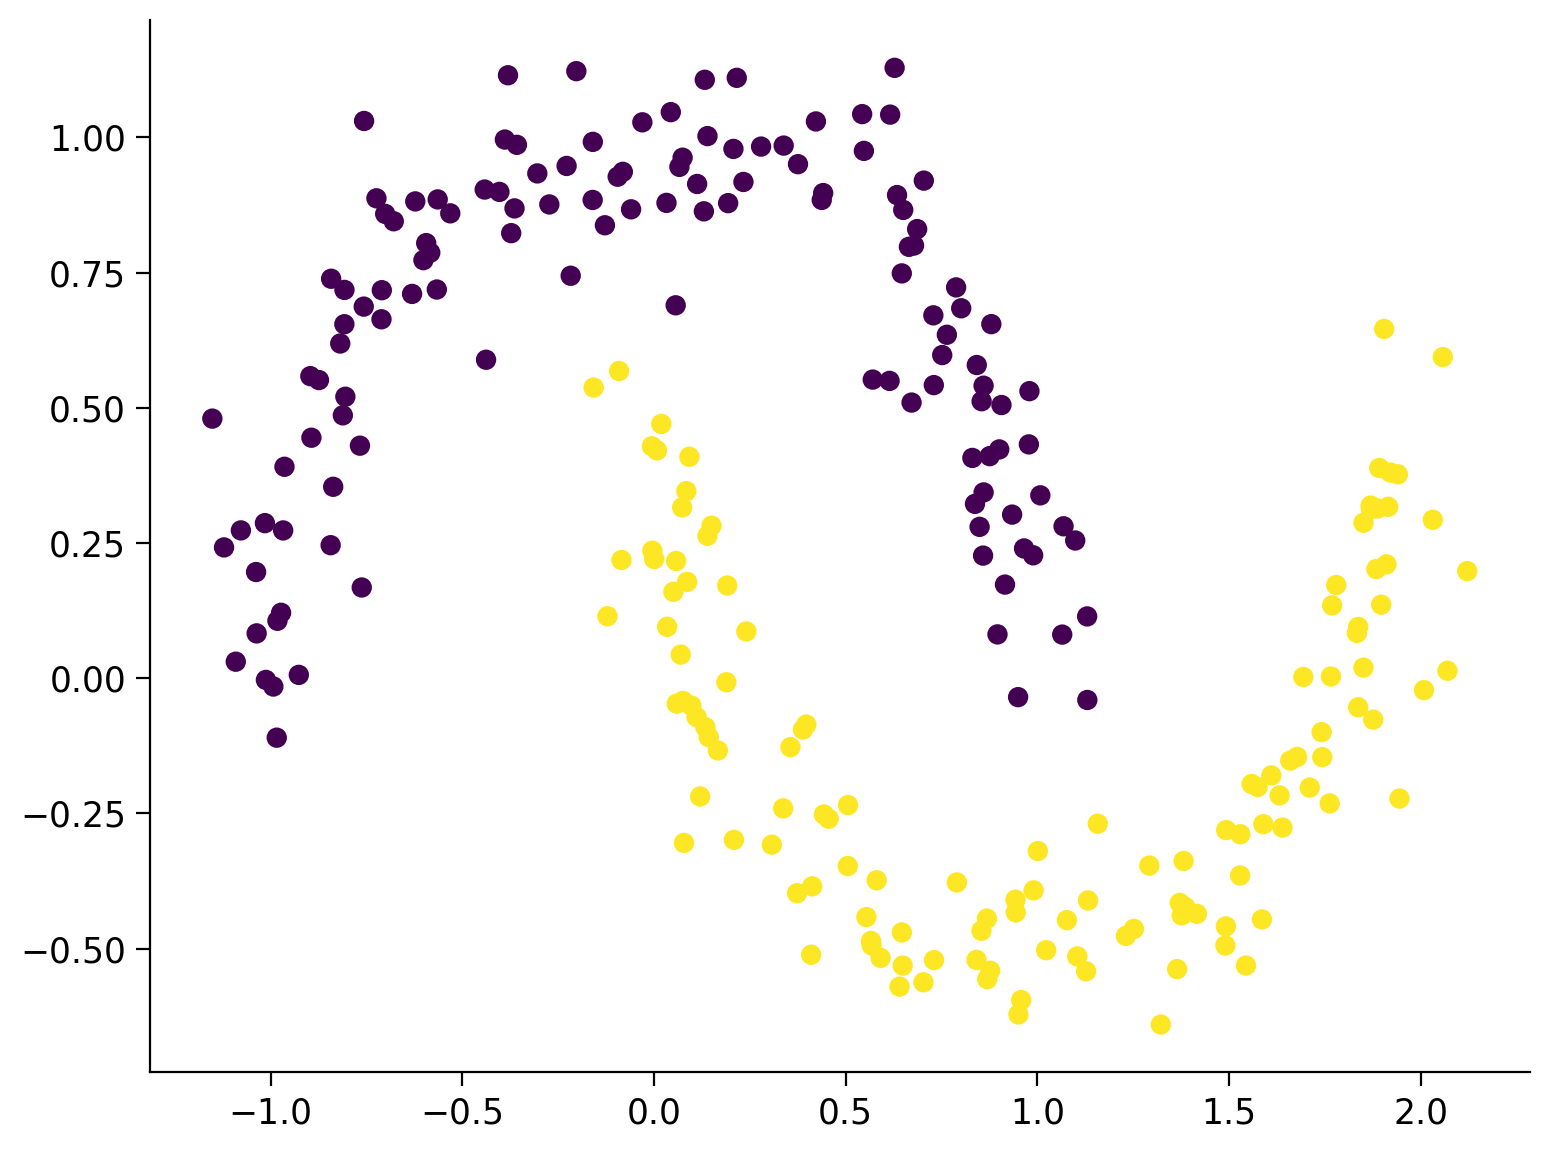
\includegraphics[scale=0.3]{Figures/NN/NNFigure1.png}


\end{subbox}
%%%%% Creating Tensors

\end{textbox}
%%%%%%%%%%%%%%%%%%%%%%%%%%%%%%%%%%%%%%%%%%%%%%%%%%
%%%%%%%%%%%%%%%%%%%%%%%%%%%%%%%%%%%%%%%%%%%%%%%%%%
\end{multicols}